\chapter{Osciladores senoidales.}\label{osc}

\section{Oscilador RC}

{\hspace{10pt}} El circuito de la figura \ref{fig1odf} es un oscilador por desplazamiento de fase de tres etapas RC. Si se diseña de modo que $C_1=C_2=C_3=C$ y que $R_1=R_2=R_b=R$ . Siendo $R_b$ la resistencia que presenta la base, es decir $R_1$ en paralelo con $R_2$ en paralelo con  la resistencia de entrada del TBJ ($r_\pi$). Bajo estas circunstancias las condiciones para oscilaciones sostenidas son las expresadas en las ecuaciones \ref{ec1odf}. De la polarización del circuito (directiva Spice \textit{.op}) se obtienen los valores: $I_{CQ}=0.9mA$, $g_m=0.0346s$ y $r_\pi=5.99k$, por lo que $R_1||R_2||r_\pi \approx 1.8K$ y $g_mR_C$ supera a la ganancia requerida por la ecuación \ref{ec1odf}.

En la figura \ref{fig2odf} se nuestra la simulación temporal de la tensión en el colector del transistor, en ella se ve una onda aproximadamente senoidal con una amplitud  de $7.95V$ pico a pico y una frecuencia de $f_o=868.6Hz$. La frecuencia teórica obtenida de la ecuación \ref{ec1odf} es de $874.72Hz$ muy similar a la hallada por simulación.  

\begin{equation}\label{ec1odf}
	f_{osc}=\displaystyle \frac{1}{2\pi RC\sqrt{6+4\displaystyle \frac{R_c}{R}}} \quad \quad y \quad \quad g_mR_C \geq 29+23\displaystyle \frac{R_C}{R}+4\left(\displaystyle \frac{R_C}{R}\right)^{2}	
\end{equation}


\begin{figure}
	\centering
	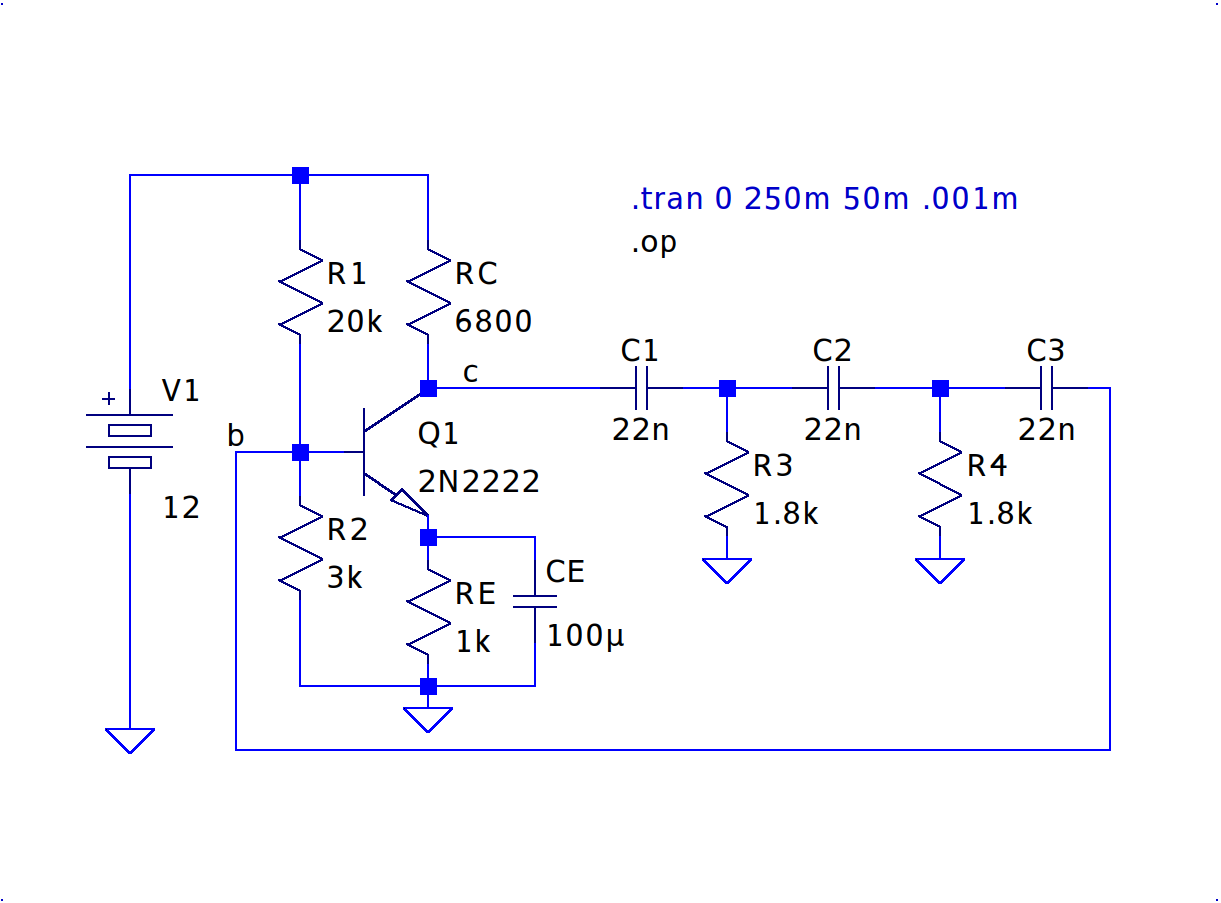
\includegraphics[width=0.8\linewidth]{figuras/despfase_circuito.png}
	\caption{Oscilador por desplazamiento de fase.}
	\label{fig1odf}
\end{figure}


\begin{figure}
	\centering
	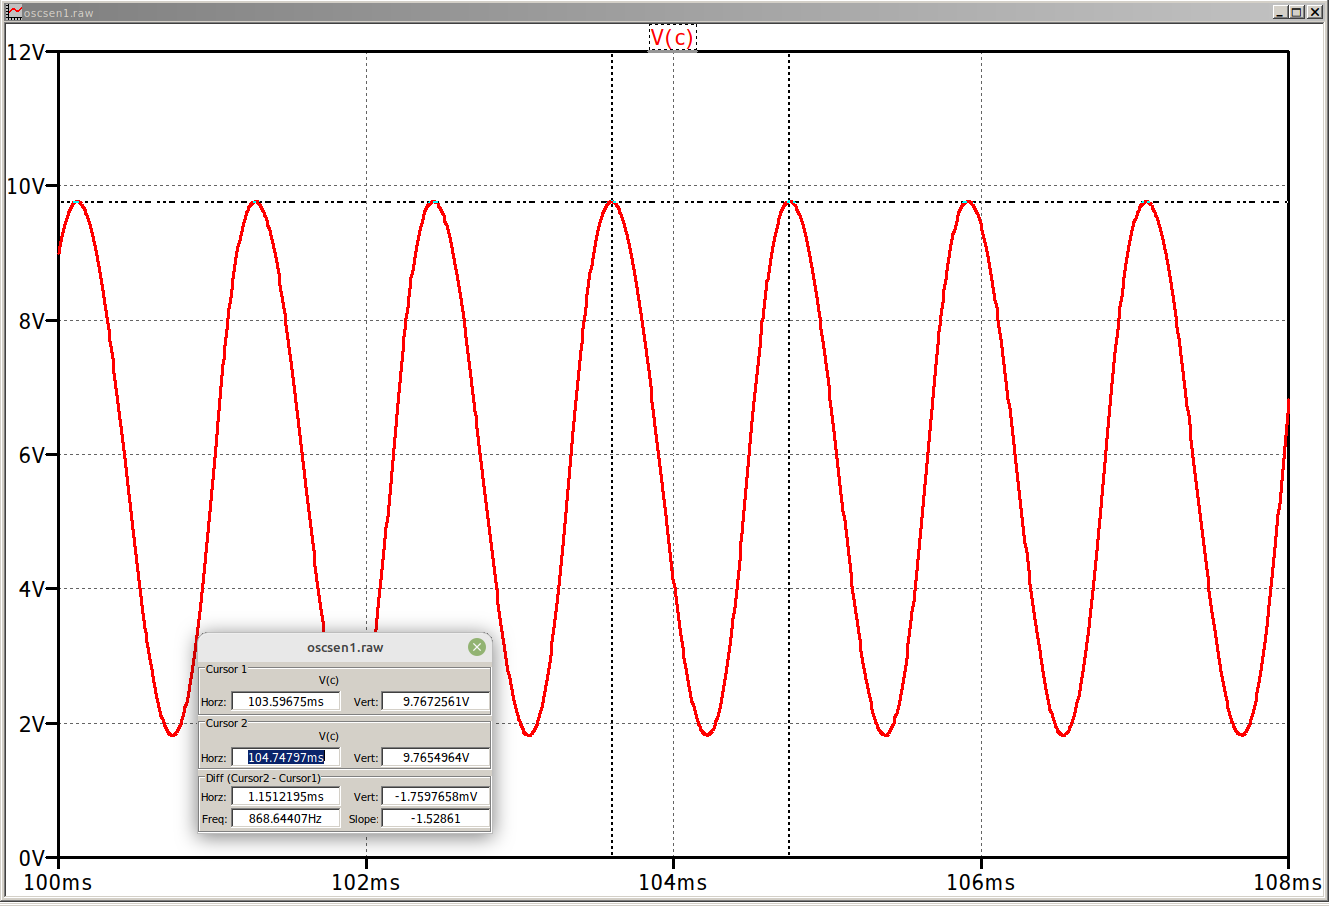
\includegraphics[width=0.8\linewidth]{figuras/despfase_curva.png}
	\caption{Simulación temporal del Oscilador de la figura \ref{fig1odf}.}
	\label{fig2odf}
\end{figure}



\section{Osciladores LC}

\begin{figure}[h]
	\centering
	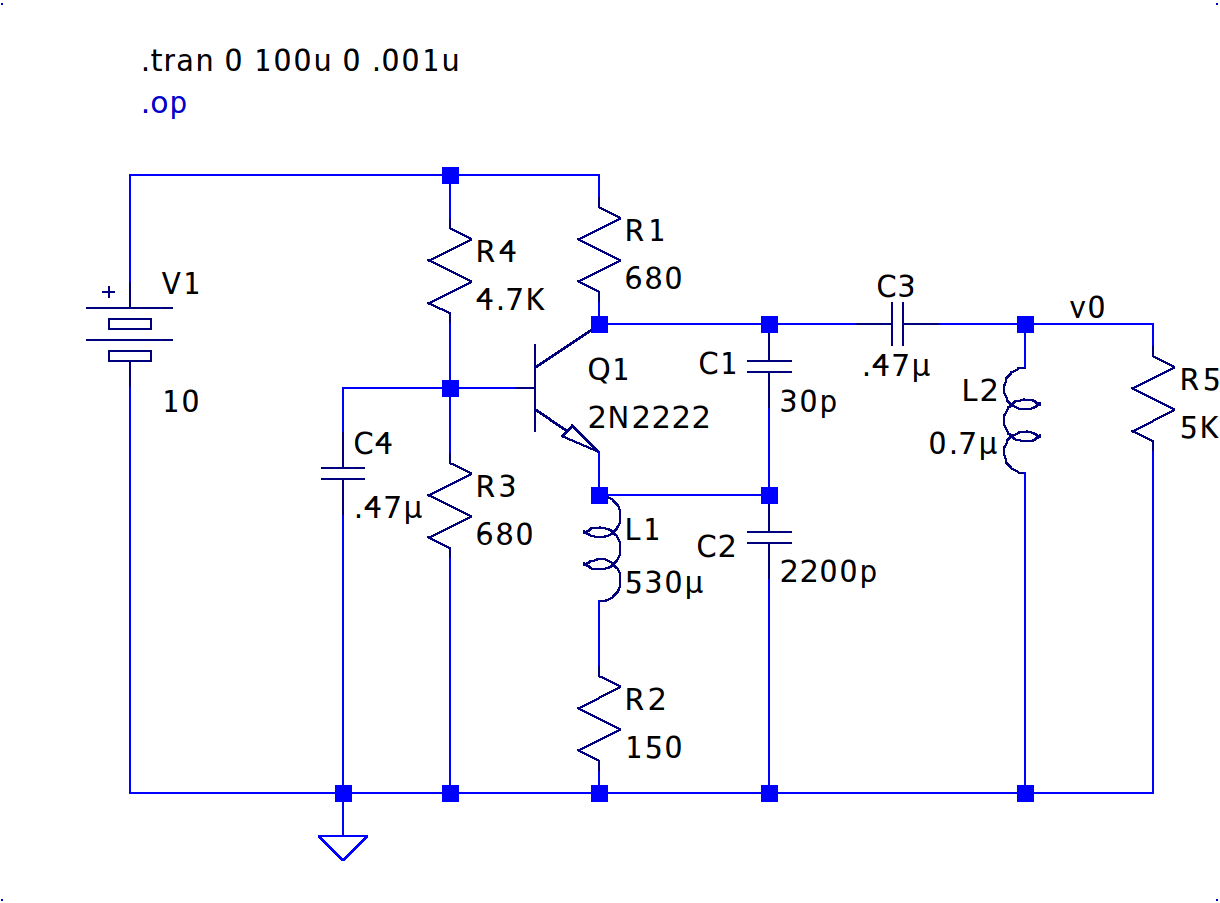
\includegraphics[width=0.8\linewidth]{figuras/lc1_circuito.png}
	\caption{Oscilador LC Colpitts.}
	\label{fig3odf}
\end{figure}



{\hspace{10pt}} El circuito de la figura \ref{fig3odf} es un oscilador LC tipo Colpitts. Los capacitores $C_3$ y $C_4$ deberían comportarse como un corto circuito y la inductancia $L_1$ como un circuito abierto  a la frecuencia de ocilación. Bajo esas condiciones los capacitores $C_1$ y $C_2$ la inductancia $L_2$ forman el circuito $\pi$ de la red de realimentación del oscilador. La teoría de osciladores indica que la frecuencia de oscilación y la ganancia requerida para oscilaciones sostenidas serían les expresadas en la ecuación \ref{ec2odf}

\begin{equation}\label{ec2odf}
	f_{osc}=\displaystyle \frac{1}{\sqrt{L_2 \displaystyle \frac{C_1C_2}{C_1+C_2}}} \quad \quad y \quad \quad g_mR_{eq} \geq \frac{C_2}{C_1}	
\end{equation}

La resistencia $R_{eq}$ es la resistencia entre colector y emisor reflejada a la frecuencia de oscilación.

En la figura \ref{fig4odf} se muestra la simulación temporal de la tensión $V_o$ y de la corriente de colector de $Q_1$. Se ve que la frecuencia de oscilación es de $31.46MHz$, la amplitud pico a pico de $V_o$ es de $\approx 2.7V$ y la corriente de colector oscila entre $1mA$ y $7.2mA$. La frecuencia teórica dada por la ecuación \ref{ec2odf} es $f_{osc}\approx 35MHz$, la diferencia se debe a los efectos que producen las capacidades $C_\pi\approx97.3p$, $C_\mu\approx3.84p$ y $C_o\approx6.5p$ obtenidas del modelo del TBJ que se deben agregar al modelo teórico para ajustar el cálculo.




\begin{figure}
	\centering
	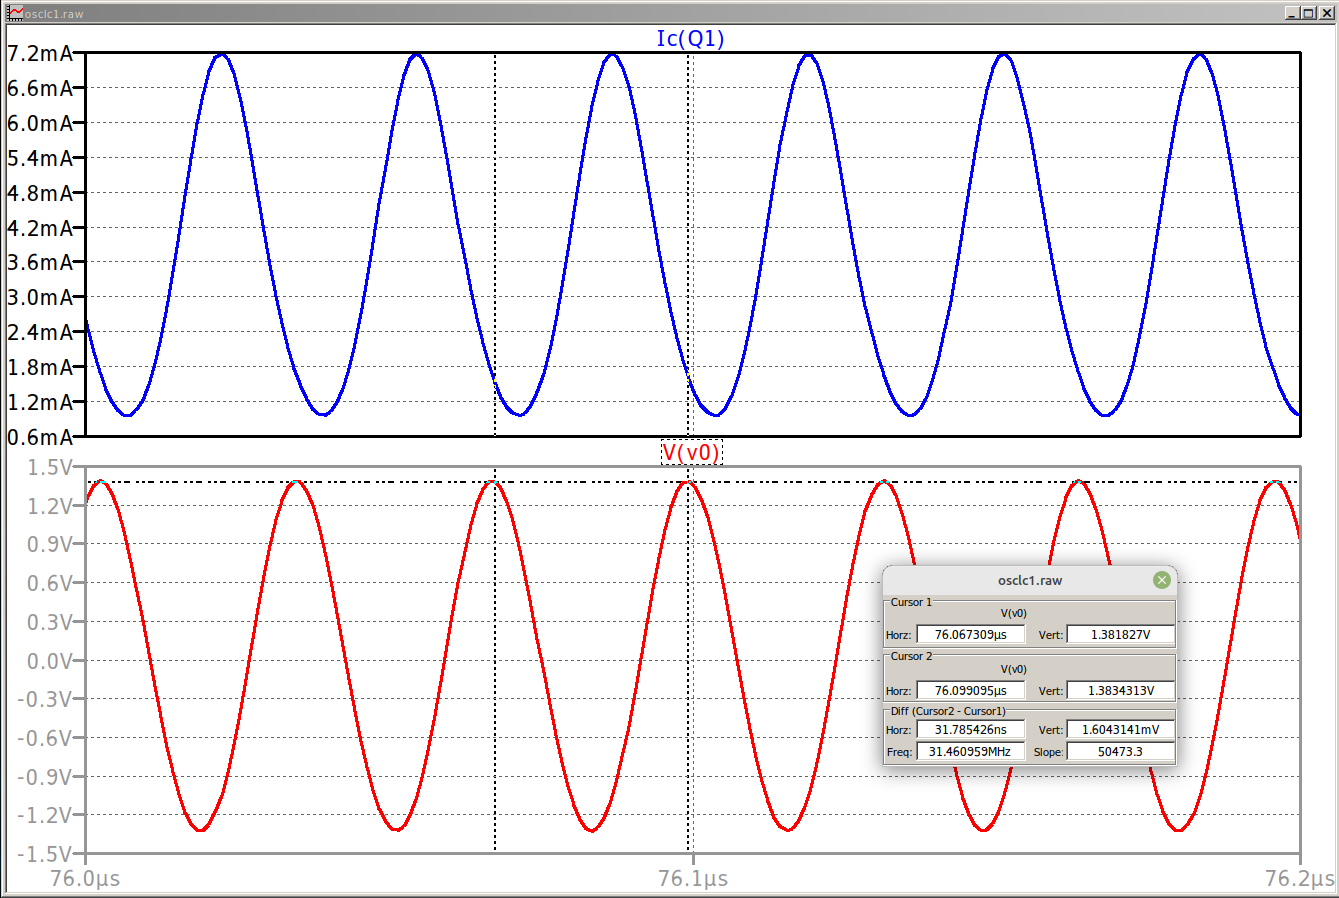
\includegraphics[width=0.8\linewidth]{figuras/lc1_curva.png}
	\caption{Simulación temporal del Oscilador de la figura \ref{fig3odf}.}
	\label{fig4odf}
\end{figure}

Los circuitos de la figura \ref{fig5odf} a) y b) son versiones de la configuración Colpitts. Según muestra la figura \ref{fig6odf} el circuito de la izquierda se comporta como un oscilador senoidal con frecuencia de oscilación de $73.7KHz$, muy cercana a la teórica, con amplitud pico a pico en el punto $V(vb)$ de $\approx 590mV$ y con variación de la corriente de colector de $Q_2$ entre $0.3mA$ y $2.4mA$. 

Bajo ciertas condiciones de diseño estos circuitos pueden presentar un comportamiento caótico, el circuito de la izquierda de la figura \ref{fig5odf} es un ejemplo de ello . Esto se muestra en las figuras \ref{fig7odf} y \ref{fig8odf}. En la primera de ellas se grafica la corriente de colector $Q_1$, discontinua en el tiempo y de amplitud cambiante y la tensión en su colector variable en el tiempo sin una periodicidad evidente. Para corroborar su comportamiento caótico se grafica en la figura \ref{fig8odf} el plano de fase de las tensiones de colector y emisor de $Q_1$, mostrando las características de un sistema de tal tipo. 



\begin{figure}
	\centering
	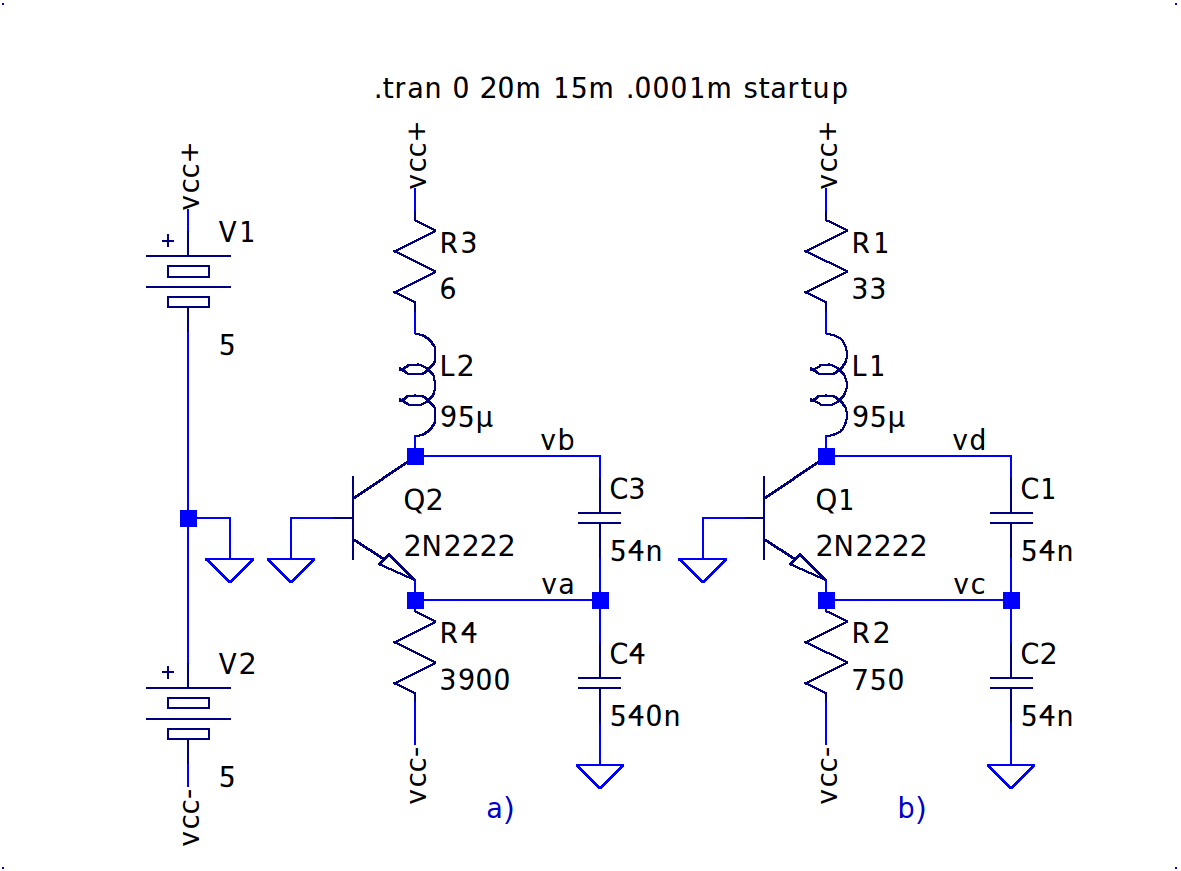
\includegraphics[width=0.8\linewidth]{figuras/lc2_circuito.png}
	\caption{Versiones del circuito tipo Colpitts.}
	\label{fig5odf}
\end{figure}

\begin{figure}
	\centering
	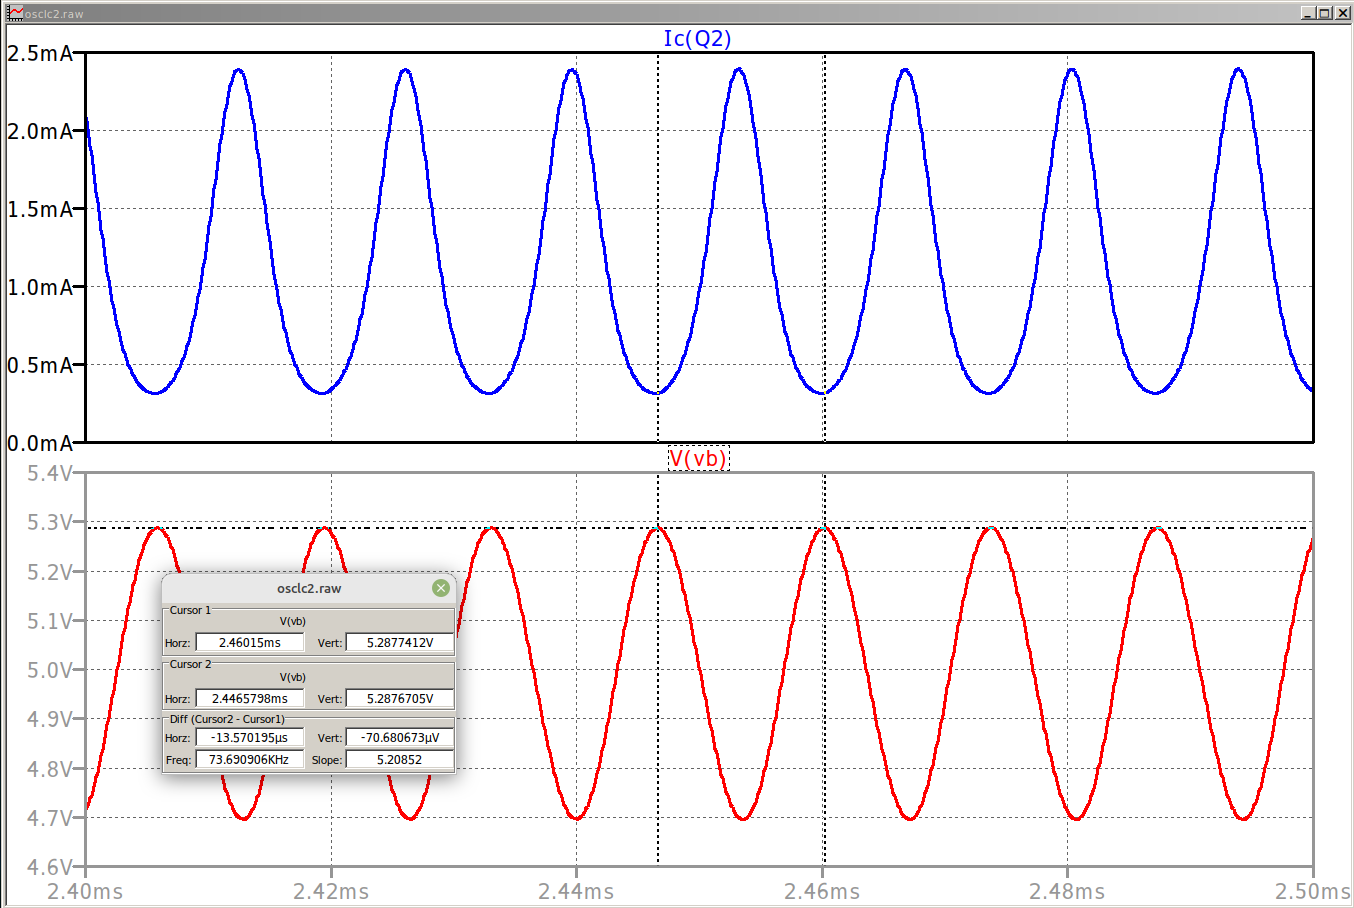
\includegraphics[width=0.8\linewidth]{figuras/lc2a_curva.png}
	\caption{Simulación temporal del Oscilador de la figura \ref{fig5odf} a).}
	\label{fig6odf}
\end{figure}

\begin{figure}
	\centering
	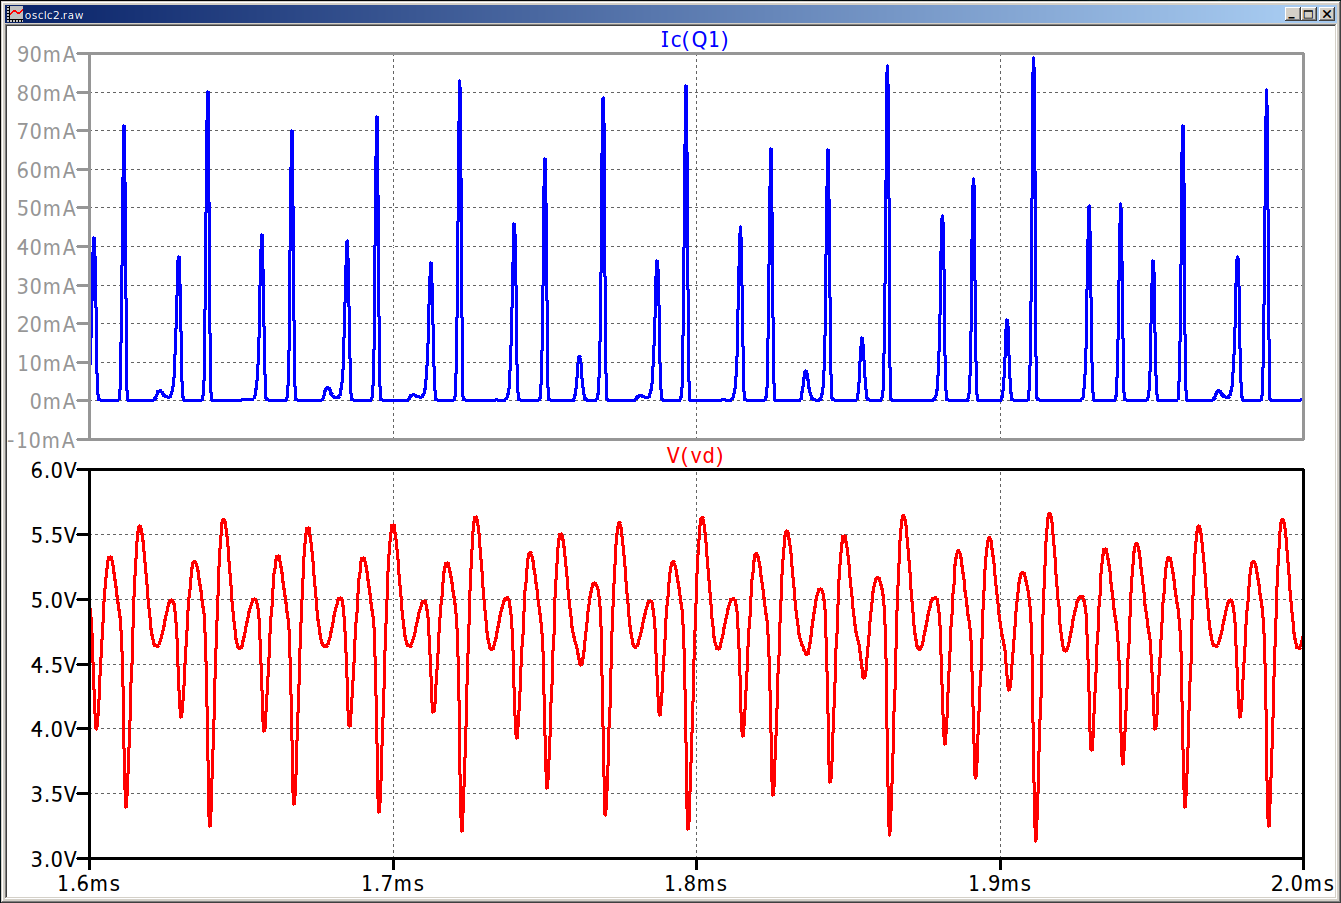
\includegraphics[width=0.8\linewidth]{figuras/lc2b_curva1.png}
	\caption{Simulación temporal del Oscilador de la figura \ref{fig5odf} b).}
	\label{fig7odf}
\end{figure}

\begin{figure}
	\centering
	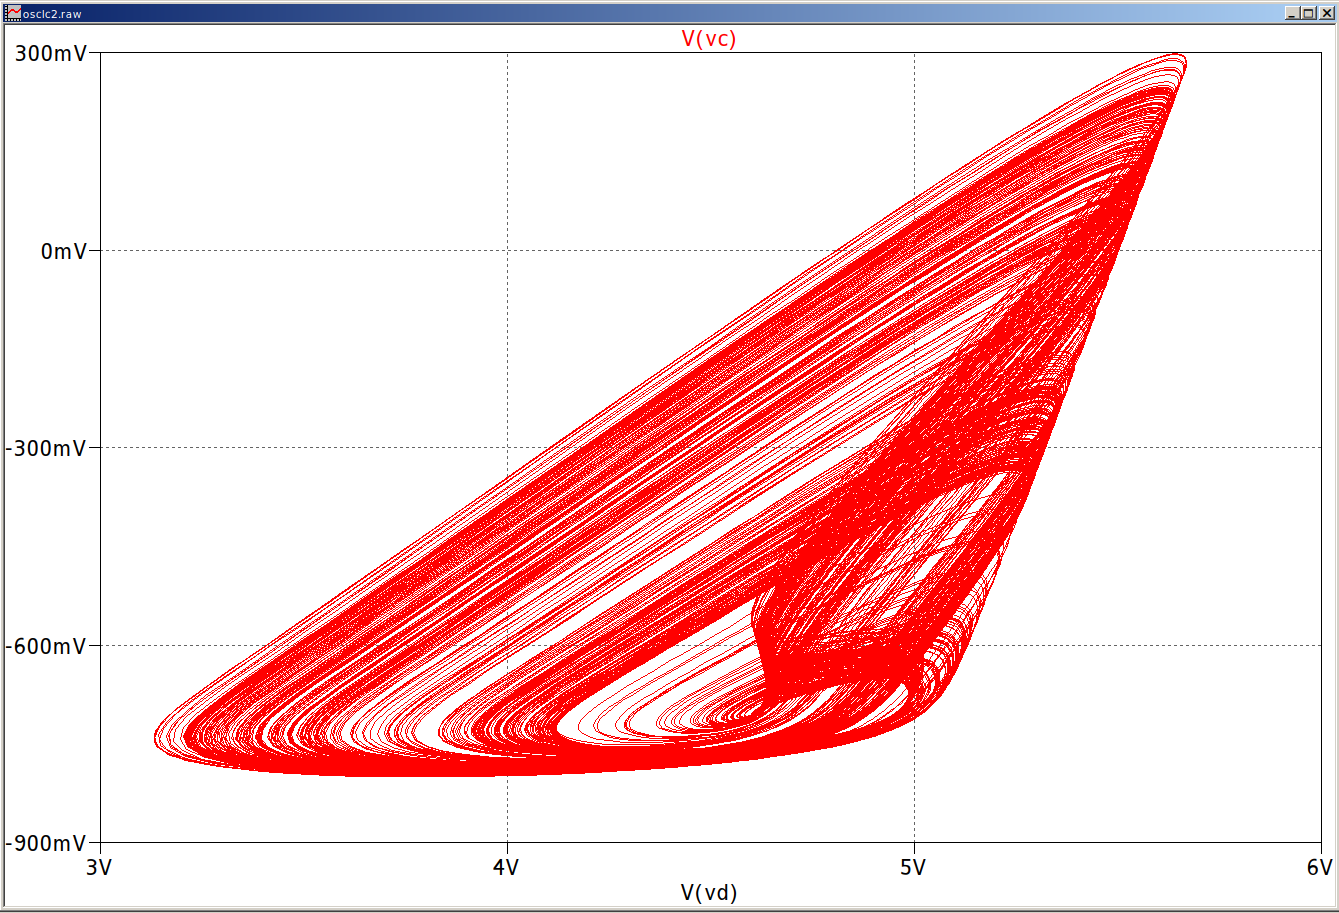
\includegraphics[width=0.7\linewidth]{figuras/lc2b_curva2.png}
	\caption{Plano de fase de las tensiones de colector y de emisor del circuito de las figura \ref{fig5odf} b).}
	\label{fig8odf}
\end{figure}


\section{Oscilador Puente de Wien}

{\hspace{10pt}} La figura \ref{fig1pw} representa el circuito Oscilador Puente de Wien básico, de la teoría de osciladores senoidales se deducen las siguientes ecuaciones  de frecuencia de oscilación y ganancia requerida para  oscilaciones sostenidas (ecuación \ref{ec1pw}).

%\begin{align*}
%	f_{osc}&=\displaystyle \frac{1}{2\pi\sqrt{R_3R_4C_1C_2}}=1KHz \\
%	1+\displaystyle \frac{R_2}{R_1}&>=1 
%\end{align*}


\begin{equation}\label{ec1pw}
	f_{osc}=\displaystyle \frac{1}{2\pi\sqrt{R_3R_4C_1C_2}}=1KHz \quad \quad y \quad \quad 1+\displaystyle \frac{R_2}{R_1} \geq 3 
\end{equation}

El circuito de la figura \ref{fig1pw} es un oscilador puente de Wien básico. La simulación temporal del circuito se muestra en la figura \ref{fig2pw} utilizando la directiva Spice \textit{.tran 0 30m 25m .001m startup}. En este caso se observa que la frecuencia de oscilación es de $\approx  1KHz$ y la amplitud está limitada por la saturación del operacional, produciéndose distorsión por recorte en los picos. Ajustando la resistencia $R_2$ se puede modificar la ganancia $1+\displaystyle \frac{R_2}{R_1}$, si se aumenta $R_2$ la ganancia aumenta y se produce mayor distorsión en los picos, si se disminuye $R_2$ la ganancia se acerca al valor límite 3, en este caso la distorsión disminuye pero se está en una zona muy crítica en la cual cualquier pequeño cambio en las condiciones del circuito puede hacer que deje de oscilar.



\begin{figure}
	\centering
	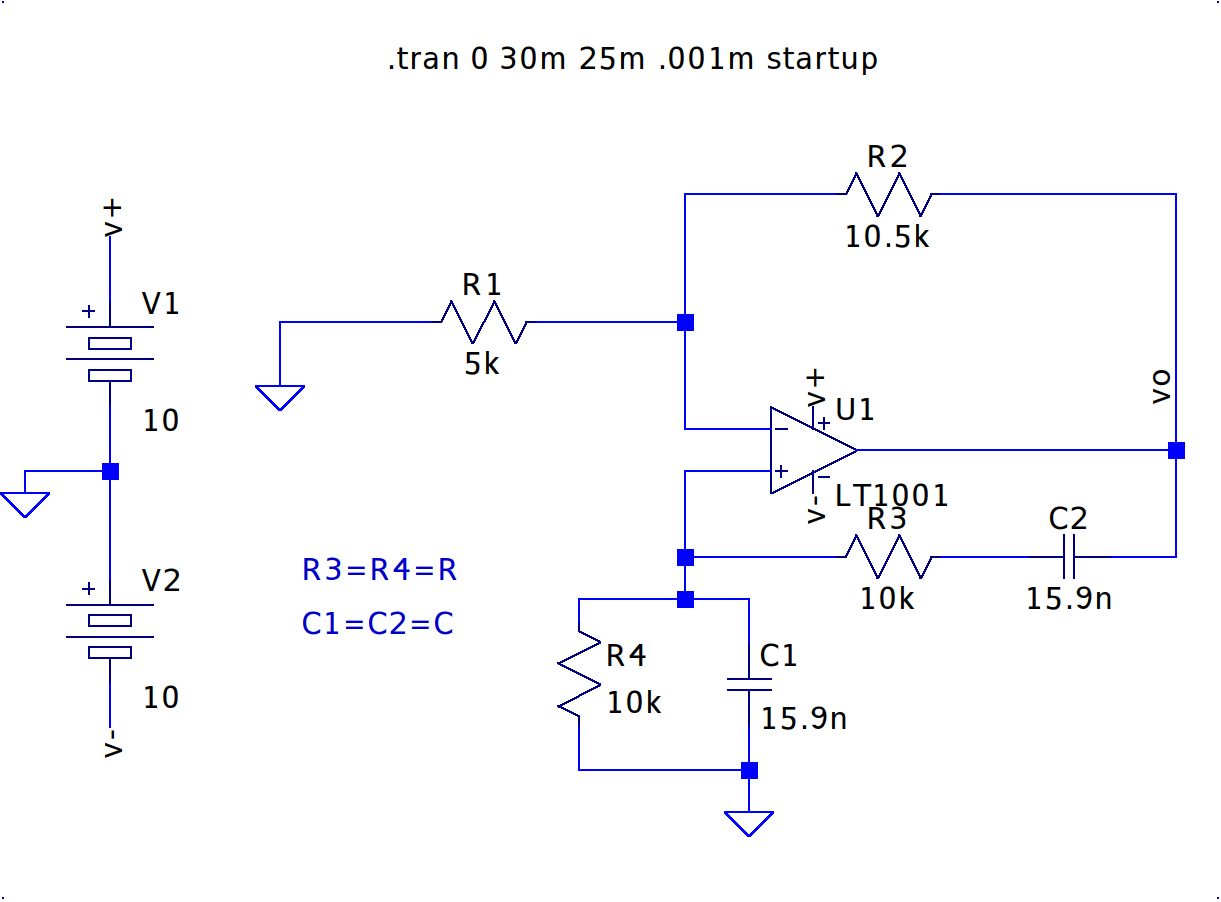
\includegraphics[width=0.8\linewidth]{figuras/wien1_circuito.png}
	\caption{Oscilador puente de Wien básico.}
	\label{fig1pw}
\end{figure}




\begin{figure}
	\centering
	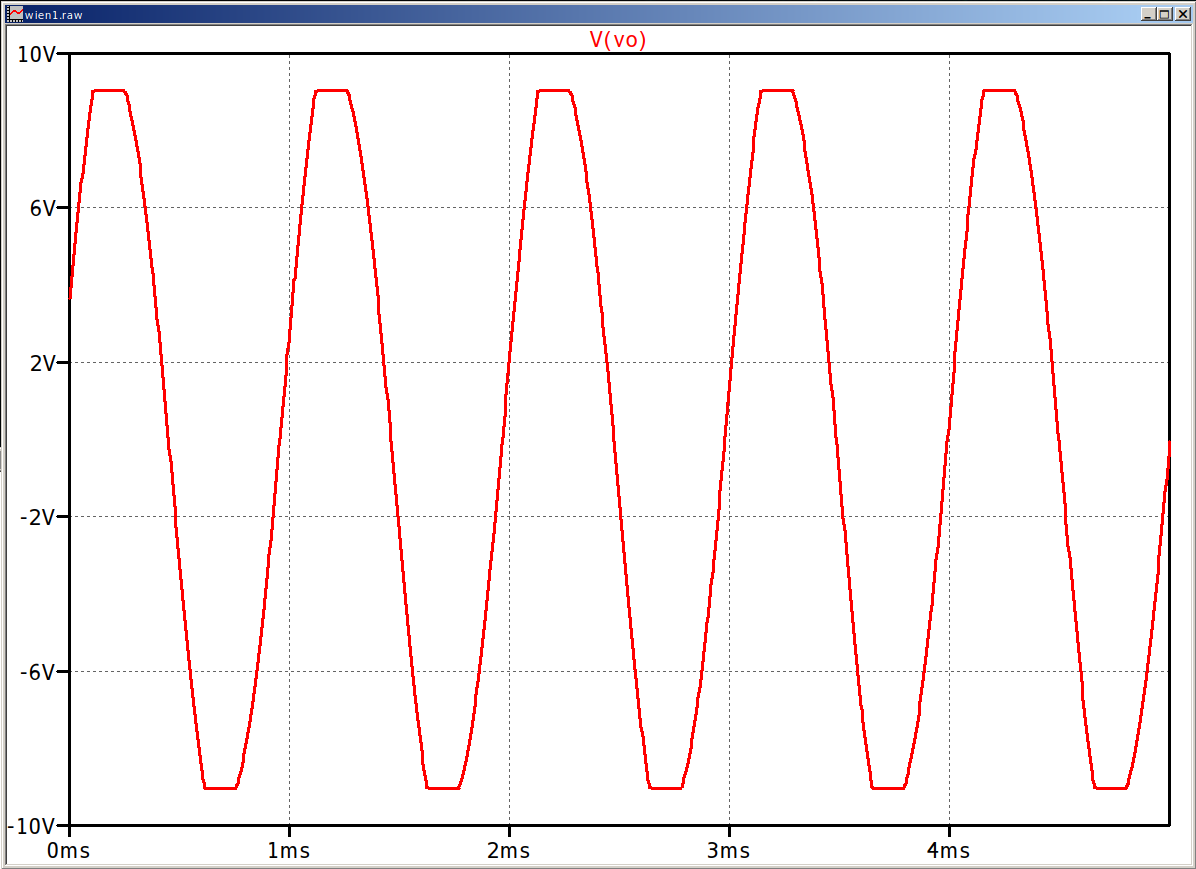
\includegraphics[width=0.8\linewidth]{figuras/wien1_curva.png}
	\caption{Simulación temporal del Oscilador puente de Wien básico.}
	\label{fig2pw}
\end{figure}


Existen diversos métodos para obtener una amplitud requerida, uno de ellos se basa en controlar en forma no lineal la resistencia en la realimentación negativa del operacional. Se busca que la resistencia en la realimentación tenga un valor tal que supere el valor teórico de oscilación para amplitudes pequeñas y otro menor al valor teórico para amplitudes mayores de modo poder limitar el crecimiento de la amplitud.

Estas ganancias dependientes de la amplitud pueden obtenerse con diodos Zener y resistencias o con diodos y resistencias como se muestra en el circuito de la figura \ref{fig3pw}. En dicho circuito, cuando los diodos $D_1$ y $D_2$ están cortados, y considerando a $R_7+R_5=1000\Omega$ como una resistencia ajustable con $0\leq a \leq 1$, la suma de las resistencias $R_1+R_5+R_6+R_7=2015 \Omega$ dará una ganancia de $1+\displaystyle \frac{2015 \Omega}{1000\Omega} > 3$ . Esta condición de ganancia >3 hará que en el arranque del transitorio la amplitud comience a crecer hasta que se enciendan los diodos (uno para cada polaridad), en el momento que los diodos están encendidos la ganancia es <3 limitando el crecimiento de la amplitud. 

En la figura \ref{fig4pw} se muestra la simulación temporal para el caso de $a=0.7$, se ve que la frecuencia es $\approx 1KHz$ y que la amplitud es de $\approx 5.5V$. En la figura \ref{fig5pw} se muestra la simulación temporal con tres valores del parámetro a, para ello se utiliza la directiva Spice \textit{.step param a list 0.6 0.7 0.8}, viendo que a medida que aumenta el parámetro a (disminuye la resistencia $R_5$) aumenta la amplitud del oscilador.




\begin{figure}
	\centering
	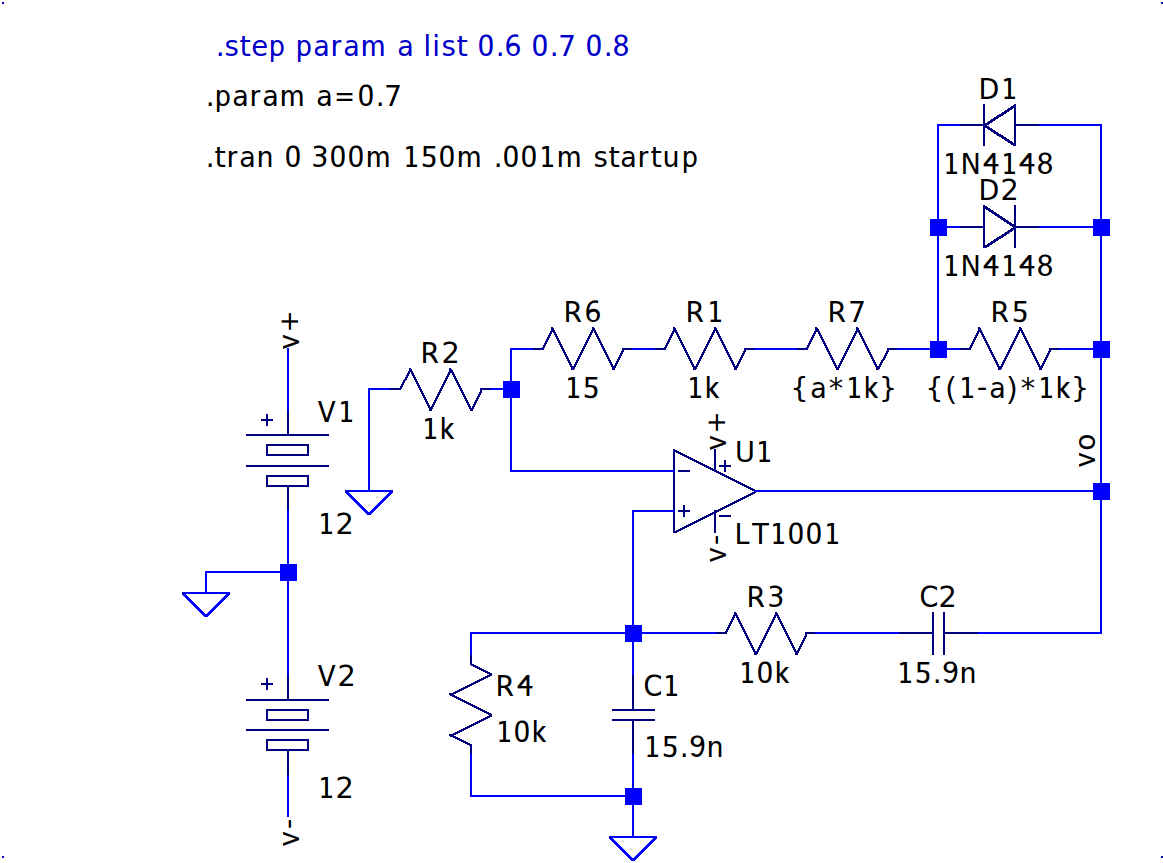
\includegraphics[width=0.8\linewidth]{figuras/wien2_circuito.png}
	\caption{Oscilador puente de Wien con control de amplitud con diodos.}
	\label{fig3pw}
\end{figure}




\begin{figure}
	\centering
	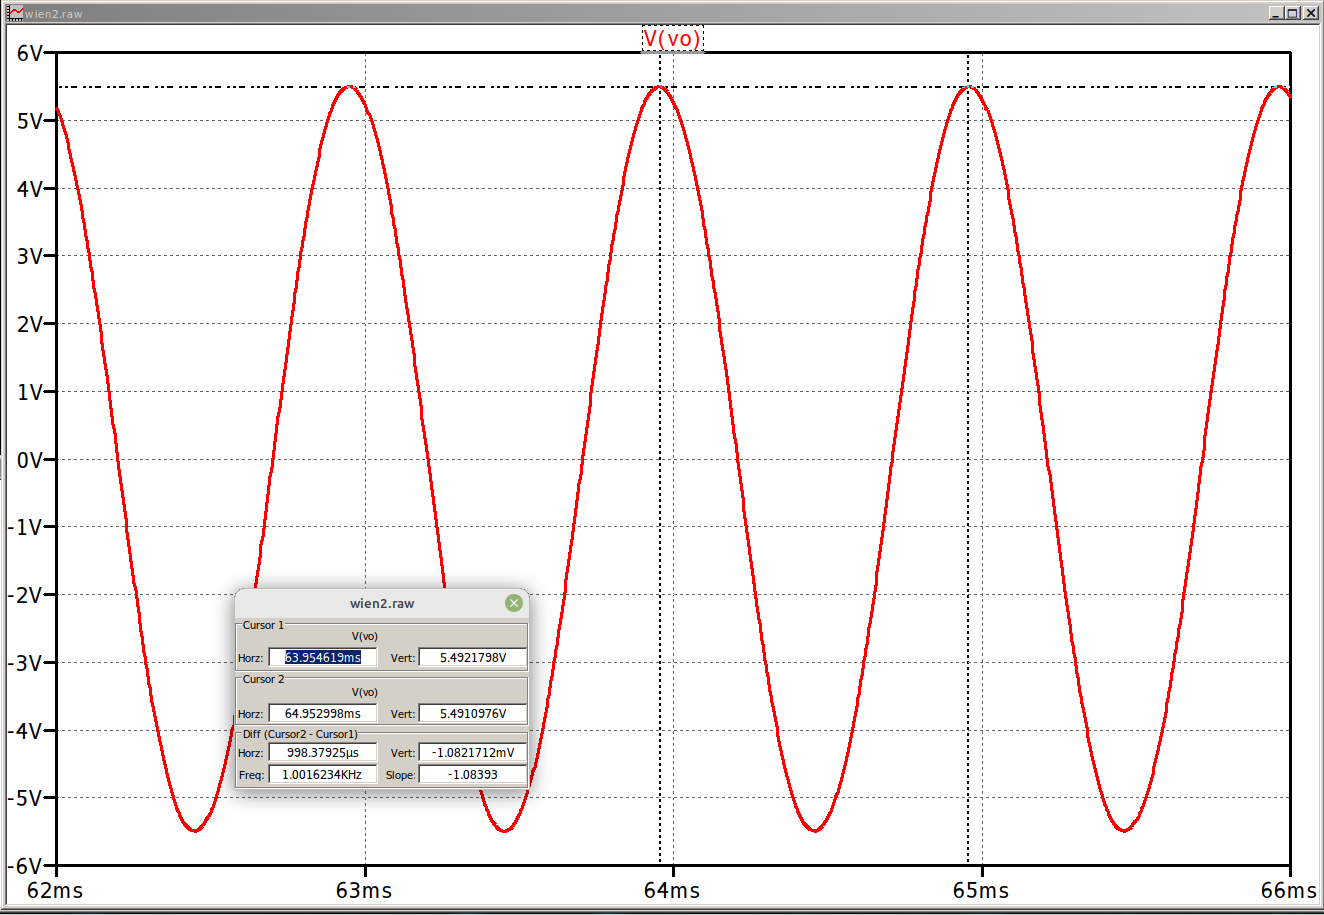
\includegraphics[width=0.8\linewidth]{figuras/wien2_curva1.png}
	\caption{Oscilador puente de Wien con control de amplitud con diodos. $a=0.7$ }
	\label{fig4pw}
\end{figure}

\begin{figure}
	\centering
	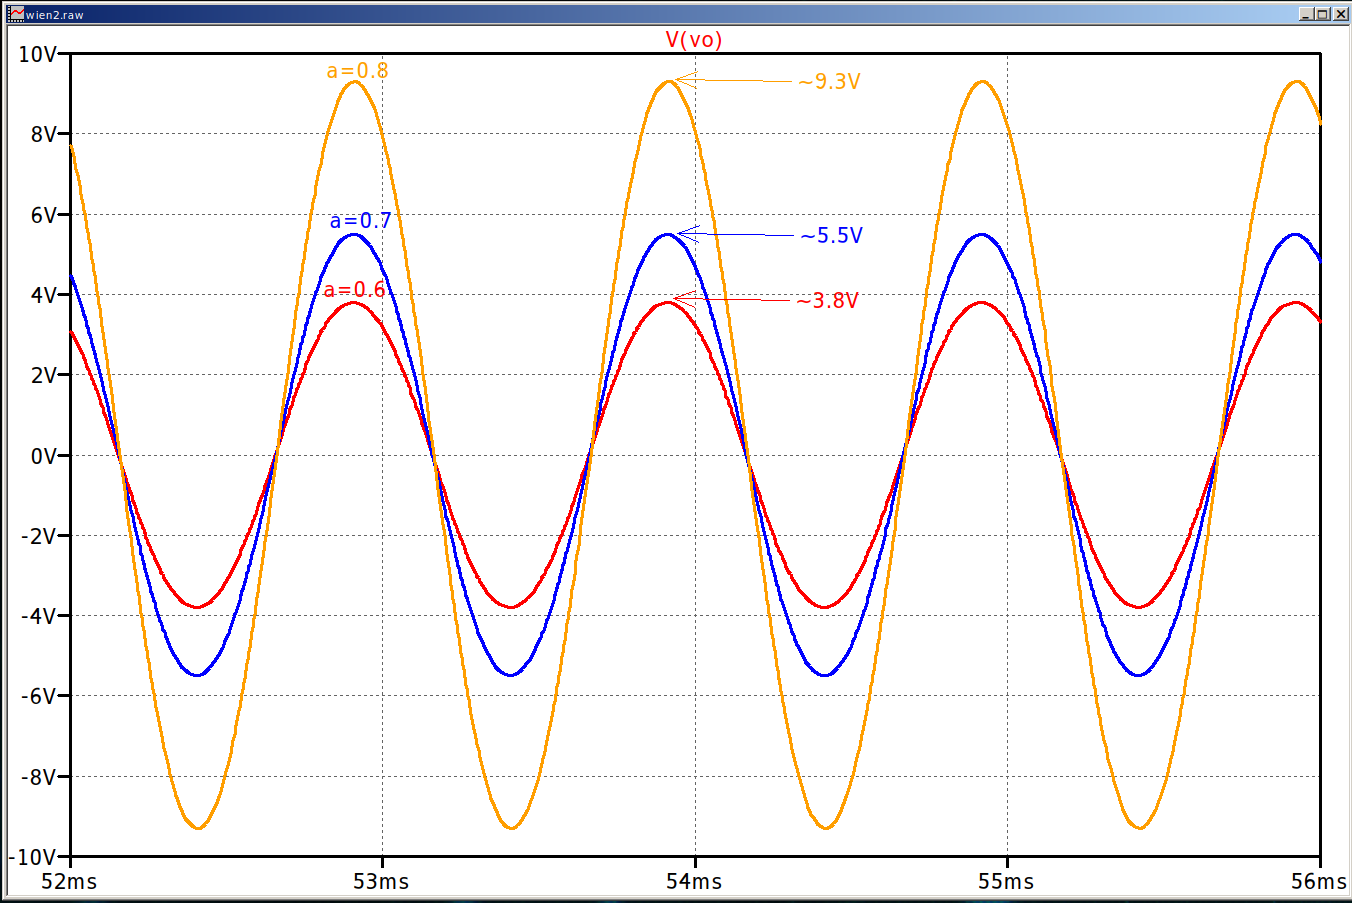
\includegraphics[width=0.8\linewidth]{figuras/wien2_curva2.png}
	\caption{Oscilador puente de Wien con control de amplitud con diodos. Con $a$ variable.}
	\label{fig5pw}
\end{figure}

\begin{figure}
	\centering
	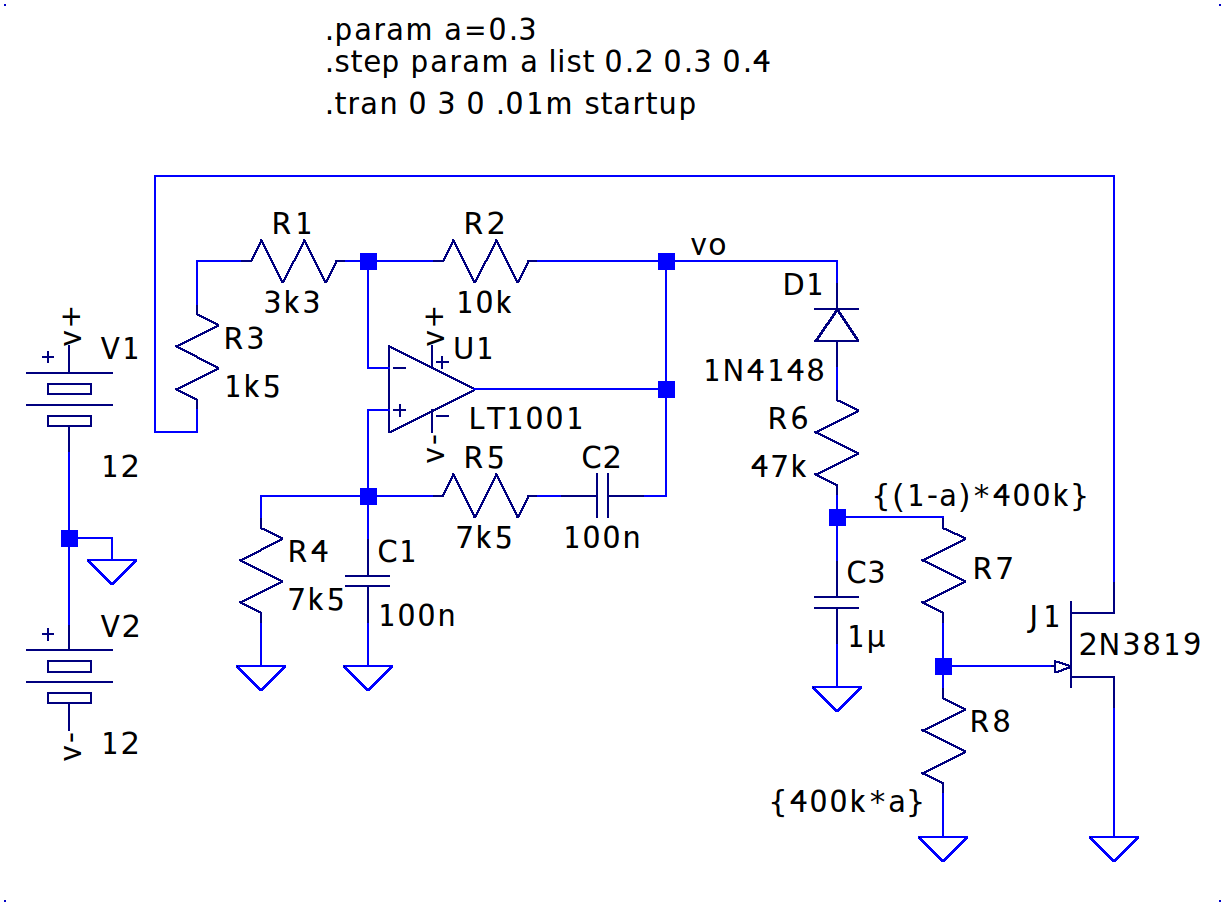
\includegraphics[width=0.8\linewidth]{figuras/wien3_circuito.png}
	\caption{Oscilador puente de Wien con control de amplitud con NJFET}
	\label{fig6pw}
\end{figure}

\begin{figure}
	\centering
	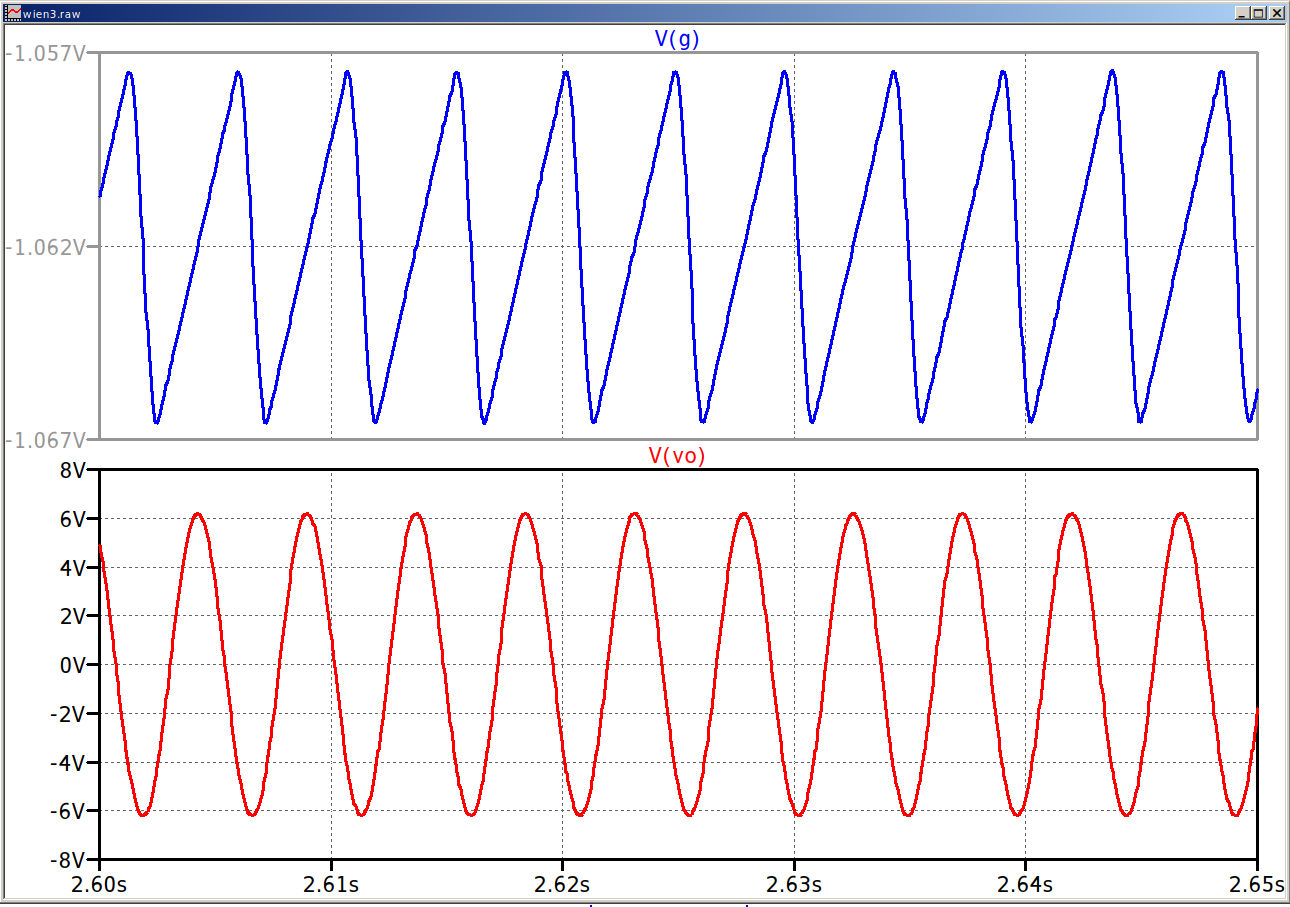
\includegraphics[width=0.8\linewidth]{figuras/wien3_curva1.png}
	\caption{Oscilador puente de Wien con control de amplitud con NJFET. $a=0.3$.}
	\label{fig7pw}
\end{figure}

\begin{figure}
	\centering
	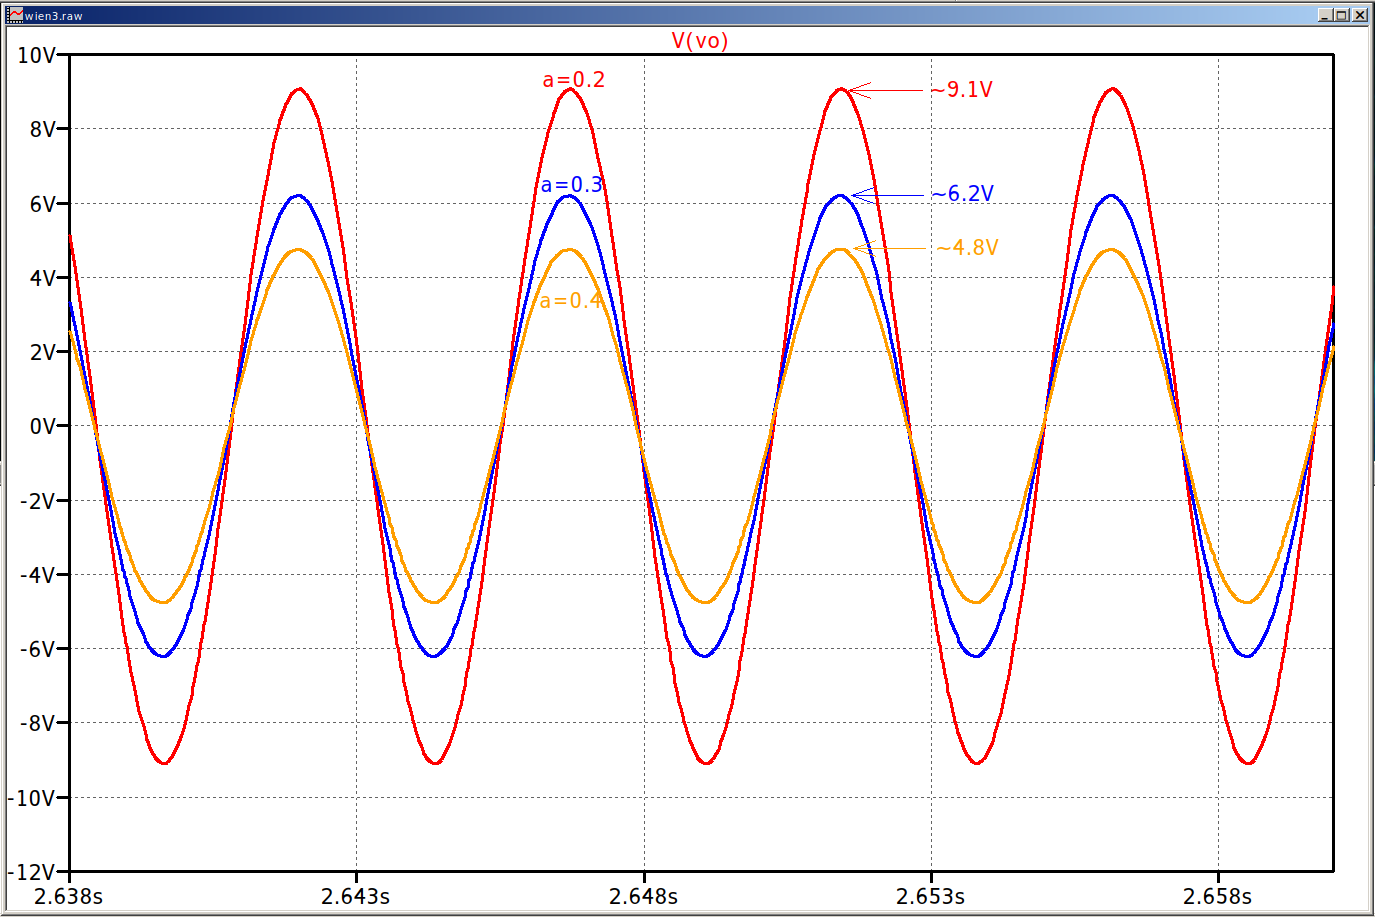
\includegraphics[width=0.8\linewidth]{figuras/wien3_curva2.png}
	\caption{Oscilador puente de Wien con control de amplitud con NJFET. Con $a$ variable.}
	\label{fig8pw}
\end{figure}


Otra manera de controlar la amplitud en un oscilador es sensar en forma continua la amplitud de salida  y modificar la etapa de ganancia del oscilador de forma adecuada para que la amplitud tienda a mantenerse en un valor establecido.

El circuito de la figura \ref{fig6pw} es un ejemplo de este caso con un oscilador Puente de Wien. En dicho circuito la ganancia del operacional está dada por $1+\displaystyle \frac{R_2}{R_1+R_3+R_{DS}}$, siendo $R_{DS}$ la resistencia que presenta el NJFET entre los terminales de Drain y Source. Es sabido que para tensiones $V_{DS}$ pequeñas el NJFET se comporta como una resistencia variable con la tensión de Gate-Source ($V_{GS}$). Cuando $V_{GS}=0$ la $R_{DS}$ es mínima, a medida que $V_{GS}$ disminuye, es decir se polariza más en inversa, la $R_{DS}$ aumenta. El sensado de la amplitud se realiza a través del circuito formado por el diodo $D_1$ las resistencias $R_6$, $R_7$ y $R_8$ y el capacitor $C_3$, que es un rectificador de onda simple negativo, de modo que la tensión negativa rectificada presente en el Gate de $J_1$ es proporcional a la amplitud de la onda de salida. En el transitorio inicial y suponiendo la tensión en $C_3$ es 0 y por lo tanto $V_{GS}$ también es 0, el NJFET presenta una $R_{DS}$ mínima, lo que implica una ganancia máxima calculada de modo que sea $>3$ para el arranque de las oscilaciones. A medida que aumenta la amplitud el Gate se va polarizando más en inversa aumentando la $R_{DS}$ y por lo tanto disminuyendo la ganancia. Hasta un punto, luego de un transitorio, en que la resistencia $R_{DS}$ es la justa para oscilaciones sostenidas. Si se supone que $R_7+R_8$ es una resistencia con punto intermedio, ajustando ese punto intermedio se puede modificar el valor de la amplitud de salida. 

La figura \ref{fig7pw} muestra la simulación del circuito con el valor del parámetro $a=0.3$, que emula el comportamiento de la resistencia con punto intermedio $R_7+R_8$. La curva de abajo es la tensión de salida del oscilador, en ella se ve que la frecuencia de oscilación coincide con la esperada ($\approx 212Hz$) y que la amplitud es de $\approx 6.2V$. La curva de arriba grafica la tensión $V_{GS}$, siendo su valor promedio $\approx -1.06V$ con un pequeño ripple proveniente de la rectificación y el filtrado correspondiente.  

En la figura \ref{fig8pw} se varía el parámetro $a$ en tres valores distintos y se muestra el cambio en la amplitud para cada caso. Valores de $a$ más bajos producen amplitudes mayores y viceversa. 




\section{Osciladores Trifásico y de Cuadratura}

\subsection{Trifásico}

{\hspace{10pt}} El circuito de la figura \ref{fig1tricua} es un oscilador trifásico implementado con operacionales. Teóricamente consta de tres etapas idénticas en las cuales $R_2=R_4=R_6=R$, $R_1=R_3=R_5=2R$ y $C_1=C_2=C_3=C$. La expresión \ref{ec1tricua} refleja la frecuencia de oscilación y la condición de ganancia para oscilaciones sostenidas.

\begin{equation}\label{ec1tricua}
	f_{osc}=\displaystyle \frac{\sqrt{3}}{4\pi RC} \quad \quad y \quad \quad Ganancia_{DC} \geq 8 
\end{equation}


Las etapas de la izquierda y del medio tienen una ganancia en continua de 2 y la etapa de la derecha tiene una ganancia algo $>2$ para producir el arranque, con control de amplitud implementado con dos diodos Zener y una resistencia.

En la figura \ref{fig2tricua} se muestra la simulación temporal de las tres salidas de los operacionales, viendo que son señales trifásicas separadas cada una $120^{\circ}$. La frecuencia obtenida es de $282.4Hz$ y su amplitud de $10.3V$, la frecuencia teórica calculada por la ecuación \ref{ec1tricua} es de $275.7Hz$, cercana a la simulada. 


\begin{figure}[ht]
	\centering
	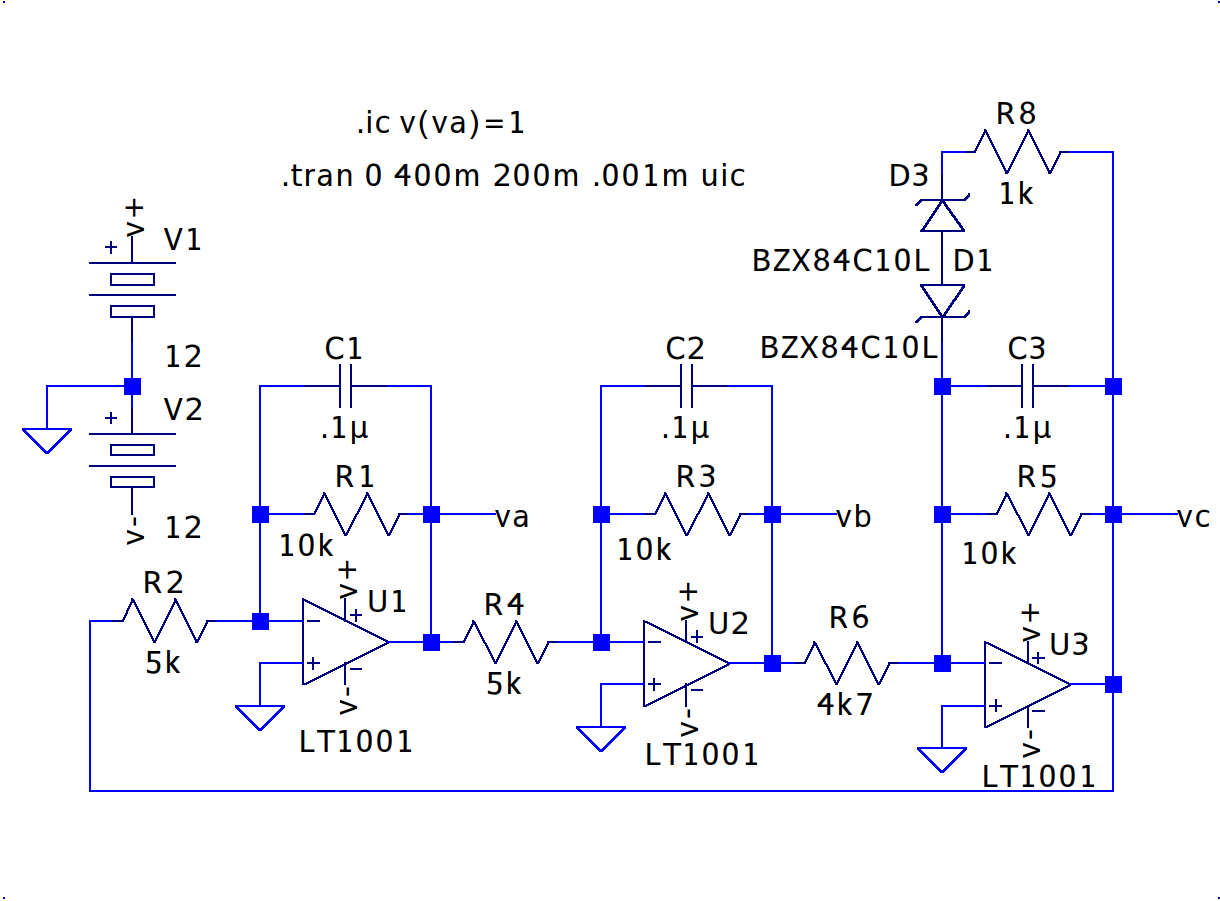
\includegraphics[width=0.8\linewidth]{figuras/trifasico_circuito.png}
	\caption{Oscilador trifásico.}
	\label{fig1tricua}
\end{figure}




\begin{figure}[ht]
	\centering
	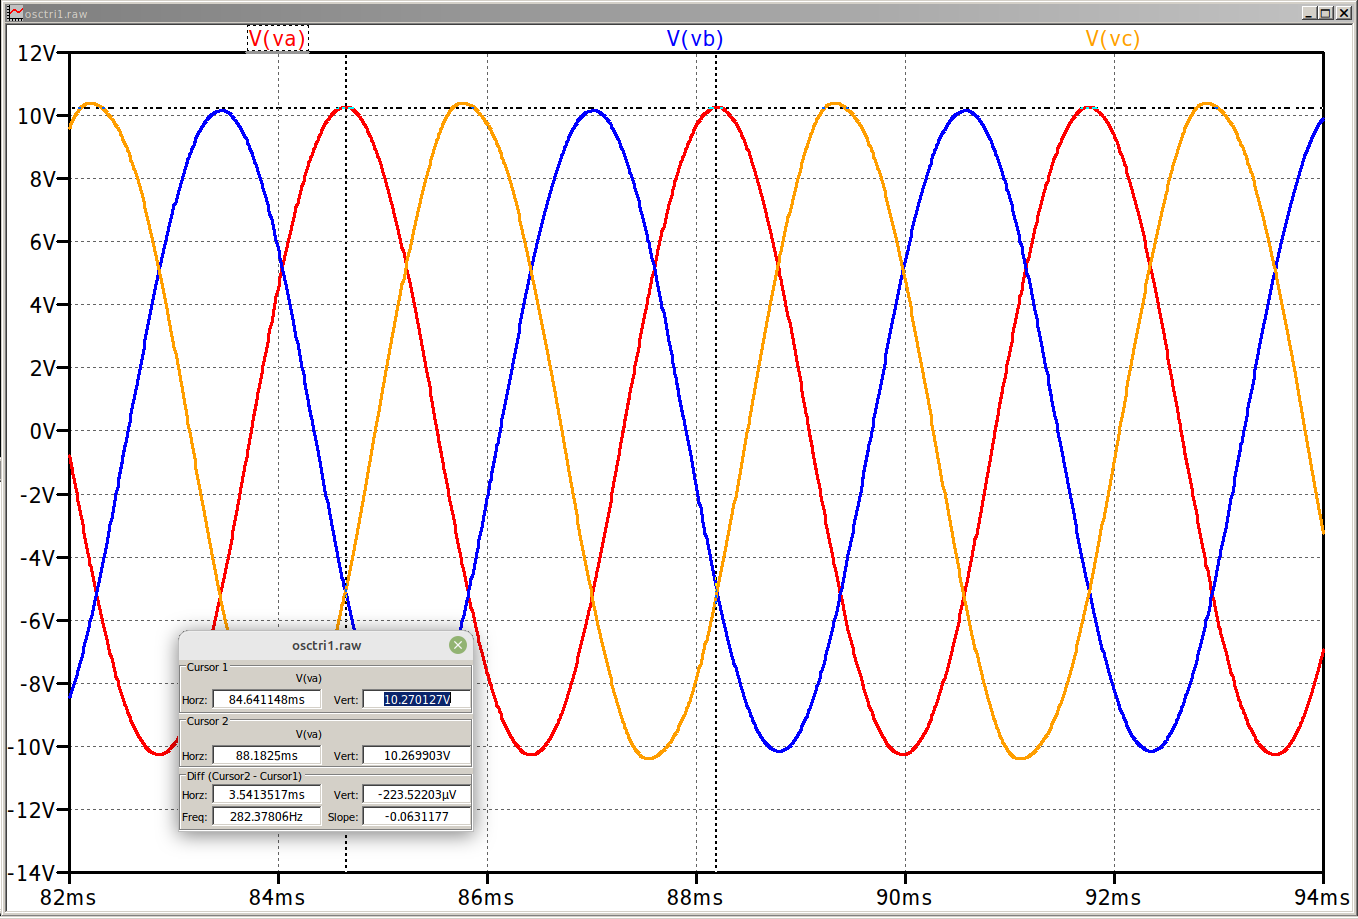
\includegraphics[width=0.8\linewidth]{figuras/trifasico_curva1.png}
	\caption{Simulación temporal del Oscilador trifásico.}
	\label{fig2tricua}
\end{figure}

\subsection{Cuadratura}

{\hspace{10pt}} El circuito de la figura \ref{fig3tricua} es un oscilador de cuadratura implementado con operacionales. Teóricamente consta de dos etapas integradoras, la de la izquierda inversora y la de la derecha no inversora, en las cuales $R_1=R$, $R_2=R_3=R_5=(R_4+R_6)=2R$ y $C_1=C_2=C$. La expresión \ref{ec2tricua} refleja la frecuencia de oscilación y la condición de ganancia para oscilaciones sostenidas.

\begin{equation}\label{ec2tricua}
	f_{osc}=\displaystyle \frac{1}{2\pi RC} \quad \quad y \quad \quad \displaystyle \frac{(R_4+R_6)}{R}  \geq 2  
\end{equation}


En la etapa de la derecha  se implementa el control de amplitud con dos diodos Zener y una resistencia. Las resistencias $R_4+R_6$ se diseñan con un valor ligeramente superior a $2R$ para producir el arranque del oscilador.

En la figura \ref{fig4tricua} se muestra la simulación temporal de las dos salidas de los operacionales, viendo que son señales separadas cada una $90^{\circ}$. La frecuencia obtenida es de $159.6Hz$ y su amplitud de $5.95V$, la frecuencia teórica calculada por la ecuación \ref{ec2tricua} es de $159.15Hz$, cercana a la simulada. 





\begin{figure}[ht]
	\centering
	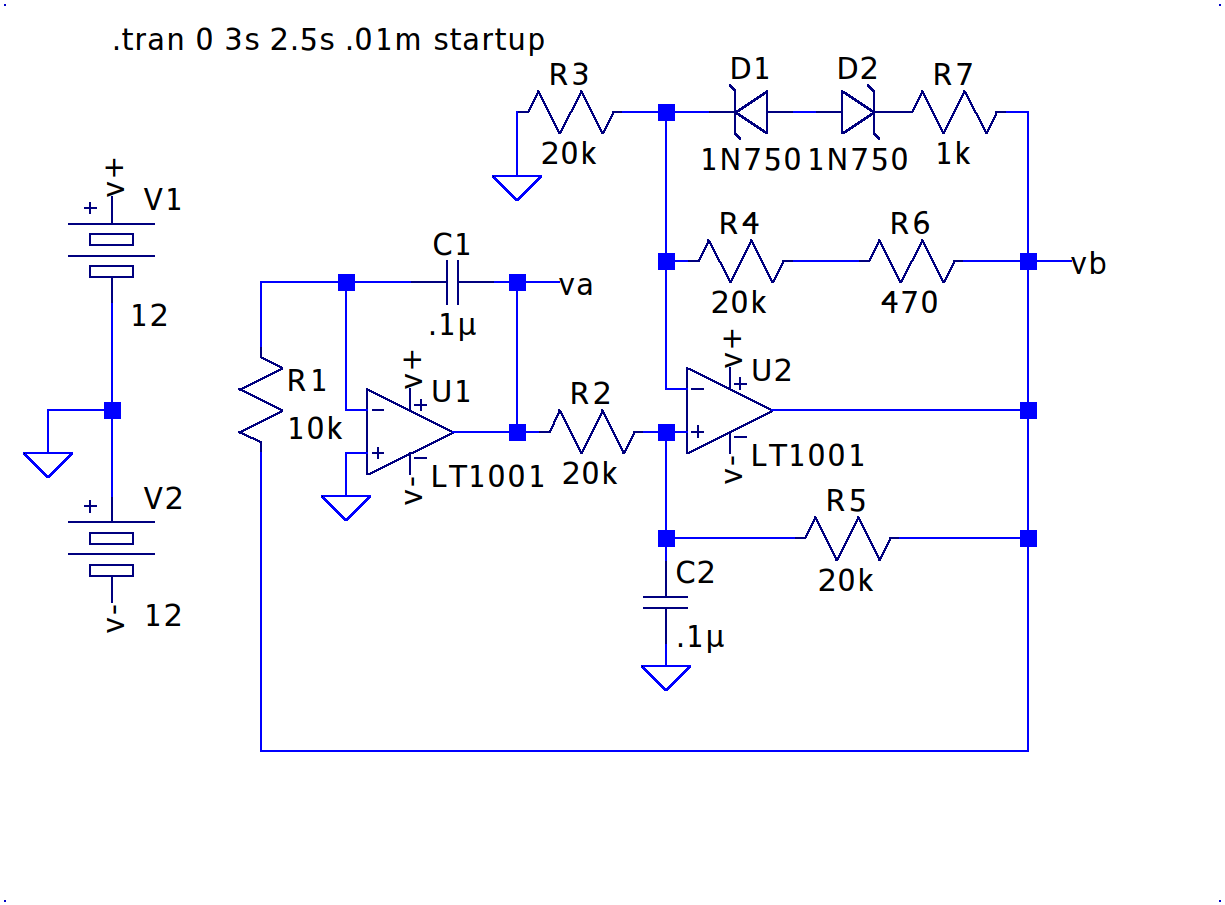
\includegraphics[width=0.8\linewidth]{figuras/cuadratura_circuito.png}
	\caption{Oscilador de cuadratura.}
	\label{fig3tricua}
\end{figure}




\begin{figure}[ht]
	\centering
	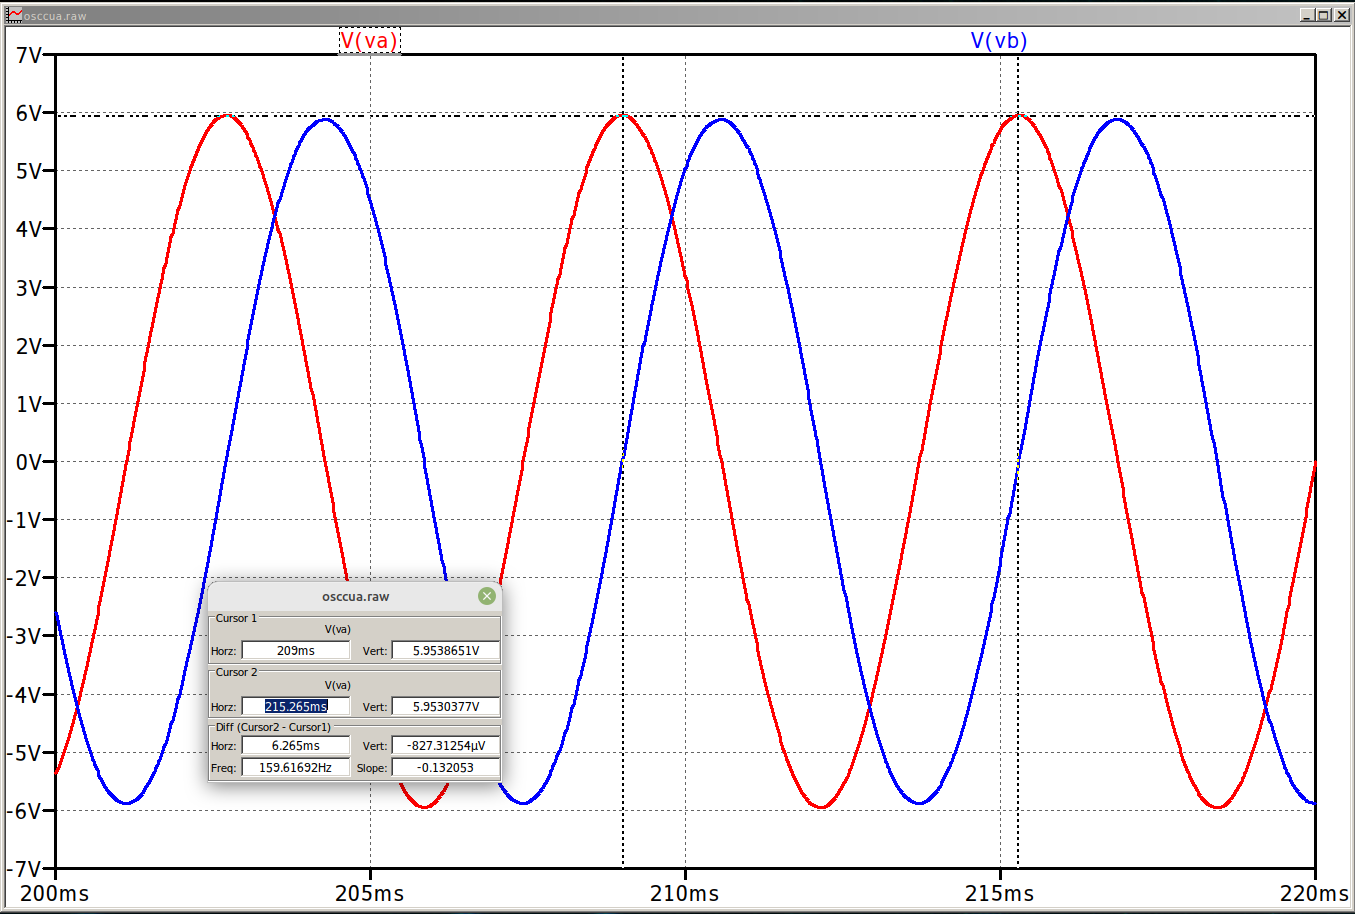
\includegraphics[width=0.8\linewidth]{figuras/cuadratura_curva1.png}
	\caption{Simulación temporal del oscilador de cuadratura. $a=0.7$ }
	\label{fig4tricua}
\end{figure}

\section{Osciladores a cristal}

{\hspace{10pt}} Los cristales piezoeléctricos de cuarzo son utilizados en circuitos osciladores en donde la estabilidad en frecuencia requerida es muy elevada. 

El LTSpice se sirve del modelo típico de un capacitor para utilizar a un cristal como parte de un circuito. Por ejemplo si se define la capacidad $C=9.95fF$ con sus correspondientes inductancia y resistencia serie de $L_s=2.55Hy$ y $R_s=640\Omega$ respectivamente y su capacidad paralelo de $C_p=2.49pF$, se obtiene el modelo de un cirstal comercial de $1MHz$. El cristal se comporta inductivamente en el estrecho margen comprendidido entre la frecuencia de resonancia serie y la frecuencia de resonancia paralelo propias del cristal. En el caso del cristal del ejemplo estas son: $f_s=0.9992MHz$ y $f_p=1.0011MHZ$.

Los cristales pueden ser utilizados en osciladores con desplazamiento de fase tipo LC en reemplazo de algún inductor del lazo de realimentación o en su frecuencia de resonancia serie en un oscilador sin desplazamiento de fase colocado también en el lazo de realimentación.

Este último caso es el mostrado en el circuito de la figura \ref{fig1cris}, en este oscilador los transistores $Q_1$ y $Q_2$ producen la amplificación, sin desfasaje, necesaria y la red formada por $R_1$, $R_2$ y $C_1$ actuando como un cristal en su resonancia serie la atenuación correspondiente. 

En la figura \ref{fig2cris} se muestra la simulación de la salida $V_o$, con una frecuencia de oscilación muy cercana a $1MHz$.



\begin{figure}[ht]
	\centering
	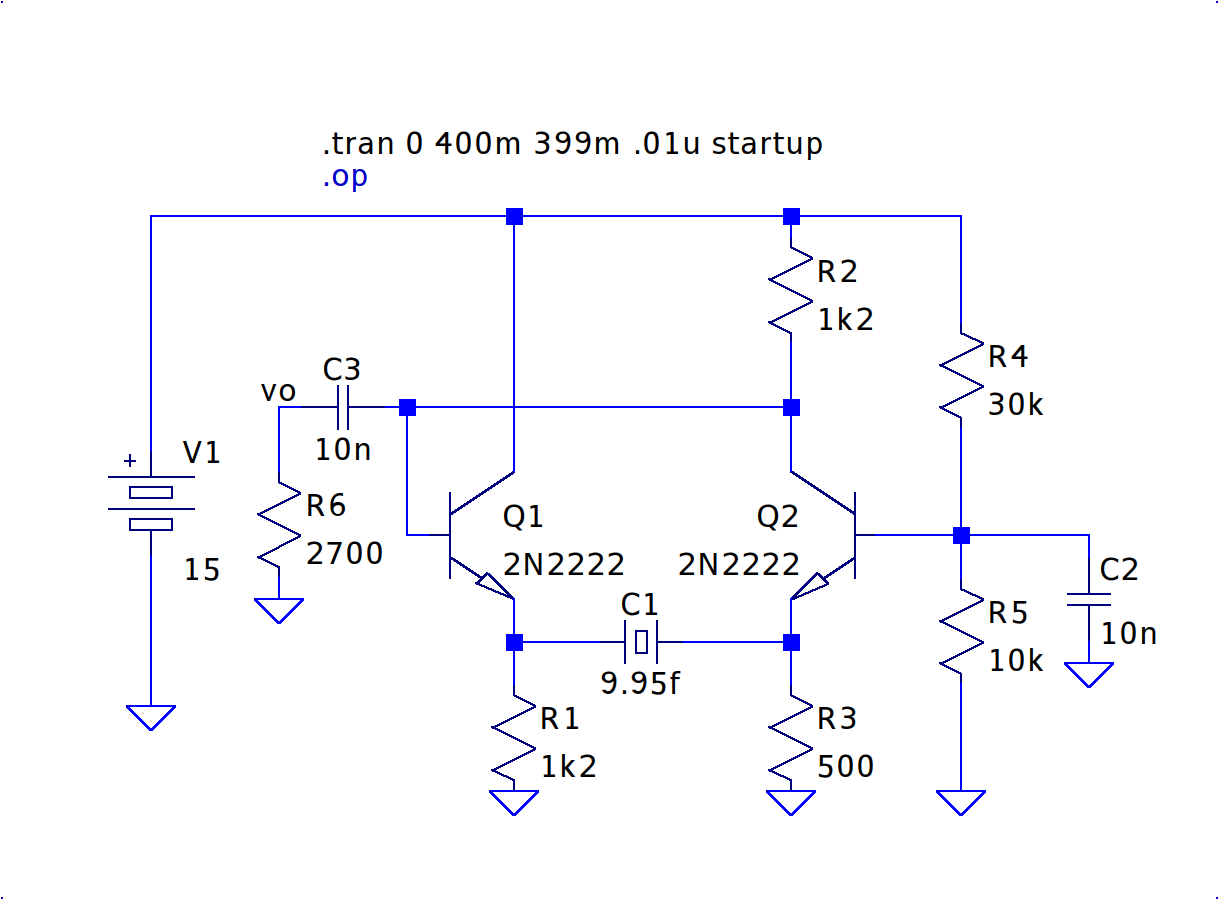
\includegraphics[width=0.8\linewidth]{figuras/osccrist1_circuito.png}
	\caption{Oscilador a cristal.}
	\label{fig1cris}
\end{figure}




\begin{figure}[ht]
	\centering
	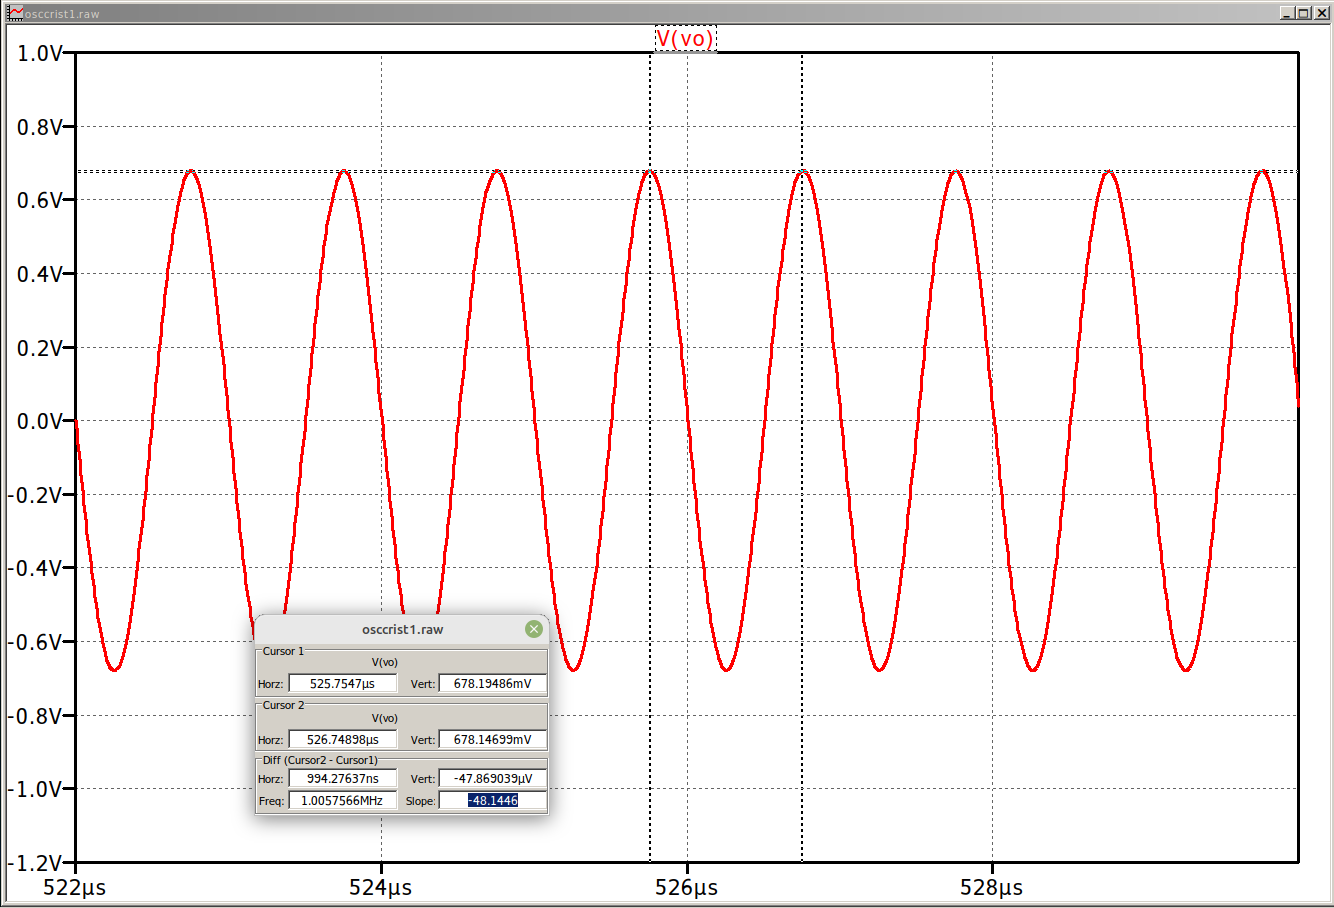
\includegraphics[width=0.8\linewidth]{figuras/osccrist1_curva.png}
	\caption{Simulación temporal del oscilador de la figura \ref{fig1cris}. }
	\label{fig2cris}
\end{figure}


